%\documentclass[10pt]{beamer}
\documentclass[10pt,handout]{beamer}
\usepackage[spanish]{babel}
% % \usepackage[backend=biber, style=authoryear-icomp]{biblatex}
\resetcounteronoverlays{exx}
\usepackage{mdframed}
\usepackage{tikz}
\usepackage{blindtext}
\usepackage{tipa}
% \usepackage{cgloss4e}
% \usepackage{gb4e}
% \usepackage{qtree}
\usepackage{cancel}
\usepackage{wrapfig}
\usepackage{soul}
\usepackage{enumerate}
\usepackage{longtable}
\graphicspath{ {./figures/} } % declaramos donde estan las imagenes
\usepackage[labelformat=simple]{subcaption} % para varias imagenes juntas
\renewcommand\thesubfigure{(\alph{subfigure})}
\usepackage[utf8]{inputenc}
\usepackage{amsmath}
\usepackage{amsfonts} % simbolos como el I de matriz identidad
\usepackage{bm}
\usepackage{graphicx} % paquete para ver imagenes
\usepackage{setspace}
\usepackage[T1]{fontenc}
\usepackage{parskip}
\usepackage{color}
\usepackage{framed}

\usetheme{Copenhagen}
\definecolor{frenchblue}{rgb}{0.0, 0.45, 0.73} % ESTE!!!!

\setbeamercolor{block body}{bg=frenchblue!50}
\setbeamercolor*{structure}{fg=frenchblue,bg=blue}
\setbeamercolor{normal text}{fg=black}
\setbeamercolor{frametitle}{bg=black}
\setbeamertemplate{frametitle}[default][center]
\setlength{\parskip}{12pt}
\useoutertheme{infolines} % me comia mucho espacio de la otra fgorma
\makeatother
\setbeamertemplate{footline}
{
  \leavevmode%
  \hbox{%
  \begin{beamercolorbox}[wd=.3\paperwidth,ht=2.25ex,dp=1ex,center]{author in head/foot}%
    \usebeamerfont{author in head/foot}\insertshortauthor
  \end{beamercolorbox}%
  \begin{beamercolorbox}[wd=.6\paperwidth,ht=2.25ex,dp=1ex,center]{title in head/foot}%
    \usebeamerfont{title in head/foot}\insertshorttitle
  \end{beamercolorbox}%
  \begin{beamercolorbox}[wd=.1\paperwidth,ht=2.25ex,dp=1ex,center]{date in head/foot}%
    \insertframenumber{} / \inserttotalframenumber\hspace*{1ex}
  \end{beamercolorbox}}%
  \vskip0pt%
}
\makeatletter
\setbeamertemplate{navigation symbols}{}
%\setbeameroption{show notes}
\setbeameroption{hide notes}


\usepackage{hyperref}

\title[Algoritmos y estructuras de datos 2]{Oblivious Data Structures}
\author[Matias Mazzanti]{Matias Mazzanti}


\institute{DC-UBA}
\date{03 de Agosto de 2022}

\titlegraphic{
\includegraphics[,height=2cm,keepaspectratio]{logo.pdf}     }
%\logo{
\includegraphics[height=2.5cm]{logo.pdf}}

\begin{document}

\begin{frame}

\maketitle

\end{frame}

\section{}
\begin{frame}
\frametitle{}
Criptografia: Codificar mensajes y operaciones por motivos de seguridad.

En particular lo aplicamos a la firma digital incremental de documentos.

Al modificar el documento incremento la firma sin necesidad de hacer una firma nueva.


El documento se divide en bloques y a cada uno se le pone una firma digital convencional.
Cada resultado de estos es una hoja del arbol.
Los nodos internos son tageados con una firma digital de sus hijos y un entero contando
la cantidad de hojas del sub arbol, que tiene de raiz a dicho nodo.
Por cada operacion basica, la firma del documento puse actualizada usando los Algoritmos
de los arboles 2-3 y recomputando las firmas de los nodos internos que fueron modificados.
Operaciones en tiempo O(logn).

Problema: No tiene privacidad. Cada actualizacion contiene informacion de las modificaciones realizadas.

Solución: Estructuras de datos indavertidas (Oblivious) $\rightarrow$ Oblivious trees.

\end{frame}
\section{}
\begin{frame}
\frametitle{}
\begin{figure}[h!]
    \centering
    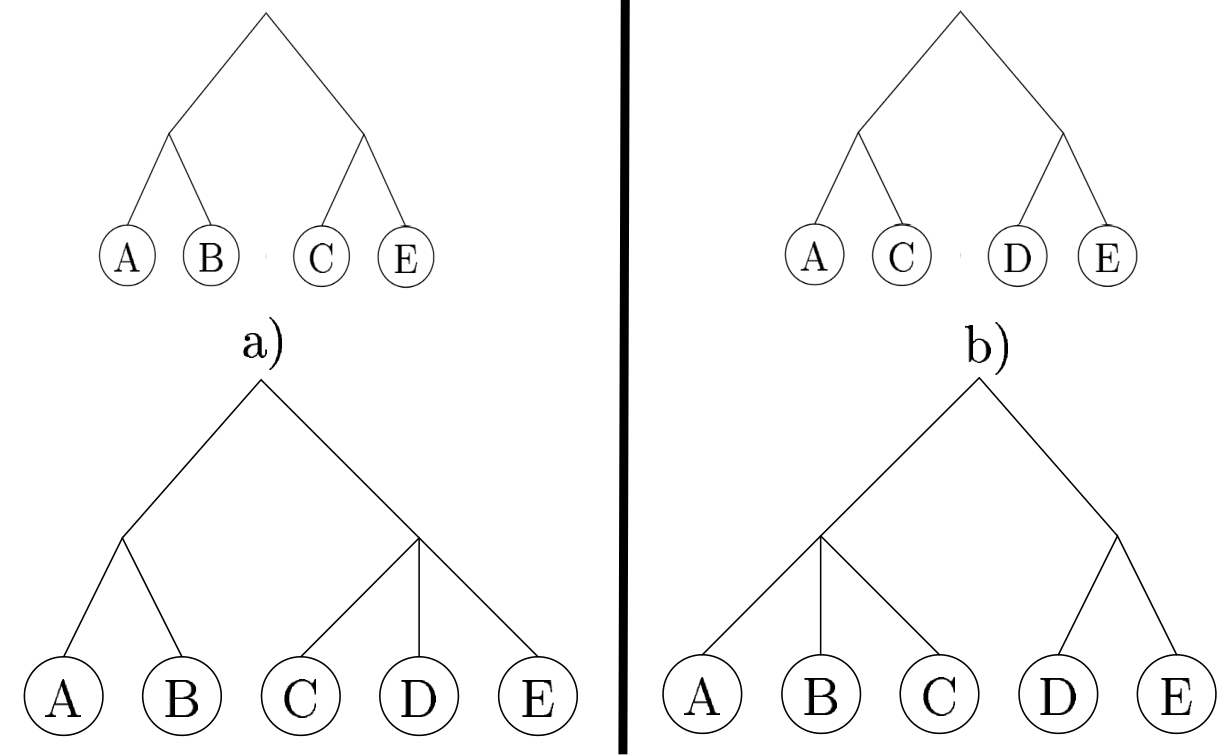
\includegraphics[scale=0.25]{2-3tree.jpg}
\end{figure}


\end{frame}


%%%%%%%%%%%%%%%%%%%%%%%%%%%%%%%%%%%%%%%%%%%%%%%%%%%%%%%%%%%%%%%%%%%%%%%%%%%%%%%%%%%%%%%%%%%%%%%%%%%%
\section{}
\begin{frame}
\frametitle{}
Nos vamos a centrar en arboes
Arboles AVL
Por que lo quiero balanceado.
\end{frame}
%%%%%%%%%%%%%%%%%%%%%%%%%%%%%%%%%%%%%%%%%%%%%%%%%%%%%%%%%%%%%%%%%%%%%%%%%%%%%%%%%%%%%%%%%%%%%%%%%%%%

\section{}
\begin{frame}
\frametitle{}
firma incremental

\end{frame}

%%%%%%%%%%%%%%%%%%%%%%%%%%%%%%%%%%%%%%%%%%%%%%%%%%%%%%%%%%%%%%%%%%%%%%%%%%%%%%%%%%%%%%%%%%%%%%%%%%%%

\section{}
\begin{frame}
\frametitle{}
Por que estos no preservan la privacidad

\end{frame}
%%%%%%%%%%%%%%%%%%%%%%%%%%%%%%%%%%%%%%%%%%%%%%%%%%%%%%%%%%%%%%%%%%%%%%%%%%%%%%%%%%%%%%%%%%%%%%%%%%%%

\section{}
\begin{frame}
\frametitle{B-tree}

\begin{columns}
    \column{0.5\textwidth}
        Arbol autobalanceado de busqueda.

Balanceado: Permite busquedas en peor caso de O(logn).

Busqueda: Mantiene orden dentro del arbol.

Utilizacion: Reducir accesos al disco, (arboles grandes que no entran en memoria principal).

Arboles B de grado M
    \column{0.5\textwidth}
        \begin{itemize}
          \item Cada noto tiene como Maximo M hijos.
          \item Un nodo que no sea hoja con k hijos contiene k-1 claves.
          \item La raiz tiene como minimo 2 hijos a menos que sea hoja.
          \item Todo nodo que no sea ni raiz ni hoja tiene al menos M/2 hijos.
          \item Todas las hojas estan al mismo nivel.
          \item Las claves estan orndeandas en cada nodo.
        \end{itemize}
\end{columns}
\end{frame}
%%%%%%%%%%%%%%%%%%%%%%%%%%%%%%%%%%%%%%%%%%%%%%%%%%%%%%%%%%%%%%%%%%%%%%%%%%%%%%%%%%%%%%%%%%%%%%%%%%%%

\section{}
\begin{frame}
\frametitle{2-3 tree}

Arboles 2-3 es un arbol B de grado 3.
\begin{itemize}
  \item Nodos con 2 hijos (alias 2-nodes) con unica clave.
  \item Nodos con 3 hijos (alias 3-nodes) con dos claves.
\end{itemize}

Insercion: Busco el lugar en orden para la nueva hoja. Si el nodo esta lleno, hago una division.
Ordeno los valores y el del medio sube al nodo padre y los extremos se separan en nuevos nodos.
Se realiza de forma recursiva en caso de necesitarse.
Caso contrario lo agrego en orden.

Borrado: Si el valor esta en un nodo interno: reemplazo el valor que quiero borrar por su
successor en ornden y borro.
Si es una hoja lo borro. Pero si el padre tiene 2 claves y tenia 3 hijos, al quedar con dos se rompe el invariante.
Bajo una de las claves del padre a uno de los nodos.
\end{frame}



%%%%%%%%%%%%%%%%%%%%%%%%%%%%%%%%%%%%%%%%%%%%%%%%%%%%%%%%%%%%%%%%%%%%%%%%%%%%%%%%%%%%%%%%%%%%%%%%%%%%

\section{}
\begin{frame}
\frametitle{Oblivious tree}

Queremos un 2-3 tree pero sin perdida de privacidad.

Modificaciones:
\begin{itemize}
  \item Permite nodos con un unico hijo, solo en caso que sea el ultimo nodo de la derecha.
  \item Toda la información de las firmas esta en las hojas.
  \item Deja de ser una estrucutra deterministica para ser probabilistica.
\end{itemize}

Cada nodo guarda su grado que es la cantidad de hijos que tine.
Tambien guarda su tamaño que es la cantidad de hojas que tiene el subarbol que tiene como
raiz al mismo.
\end{frame}


%%%%%%%%%%%%%%%%%%%%%%%%%%%%%%%%%%%%%%%%%%%%%%%%%%%%%%%%%%%%%%%%%%%%%%%%%%%%%%%%%%%%%%%%%%%%%%%%%%%%

\section{}
\begin{frame}
\frametitle{Estructura de datos inadvertidas}

Definiciones:

Un conjunto S de algoritmos que implementan un cierto conjunto de operaciones sobre el arbol de busqueda es
\texttt{Oblivious} si dada dos secuencias de operaciones $p_i$ y $q_i$ generan un arbol con una secuencias
de valores L y ambos tienen misma distribucion de probabilidad de salida.


Vamos a tener
\begin{itemize}
  \item \texttt{Crear}(L): Construye un nuevo arbol de busqueda con los valores de la secuencia L en las hojas.
  \item \texttt{Insertar}(b,i,T): Inserta una nueva hoja con valor b en la posicion i-esima del arbol T.
  \item \texttt{Borrar}(i,T): Remueve la hoja i-esima del arbol T.
\end{itemize}

Condicion para ser inadvertido.

Insertar(b,i,Crear($L_1$)) tiene la misma distribucion de probabilidad que Crear($L_2$), donde $L_{2}$
se obtiene al insetar en $L_{1}$ el elemento b en la i-esima posicion.

Borrar(i, Crear($L_{1}$)) tiene la misma distribucion de probabilidad que Crear($L_2$), donde $L_{2}$
se obtiene al sacar en $L_{1}$ el elemento en la i-esima posicion.


\end{frame}

%%%%%%%%%%%%%%%%%%%%%%%%%%%%%%%%%%%%%%%%%%%%%%%%%%%%%%%%%%%%%%%%%%%%%%%%%%%%%%%%%%%%%%%%%%%%%%%%%%%%

\section{Algoritmos}
\begin{frame}
\frametitle{Creacion}

\texttt{Crear}(L): Crea un nuevo arbol. Bottom-up

  L: Lista de claves.

  Tiempo: O(n)

  Se inicia con todas las claves en las hojas en orden dado.
  Y se arma el arbol de abajo arriba, izquierda a derecha.

\begin{itemize}
  \item Se inicia con la primer clave.
  \item Se obtiene un valor random d={2,3}.
  \item Si en el nivel que estoy tengo esa cantidad de nodos, los hago hijos de
    un nodo padre del nivel superior.
  \item Si no hay esa cantidad, d=cantidad de nodos, y los hago hijos de un nodo
    padre del nivel superior.
  \item Finalizo al no tener mas nodos (raiz).
\end{itemize}

\end{frame}

%%%%%%%%%%%%%%%%%%%%%%%%%%%%%%%%%%%%%%%%%%%%%%%%%%%%%%%%%%%%%%%%%%%%%%%%%%%%%%%%%%%%%%%%%%%%%%%%%%%%

\begin{frame}
\frametitle{Ejemplo creacion}

  \only<1>{\begin{figure}[h!]
    \centering
    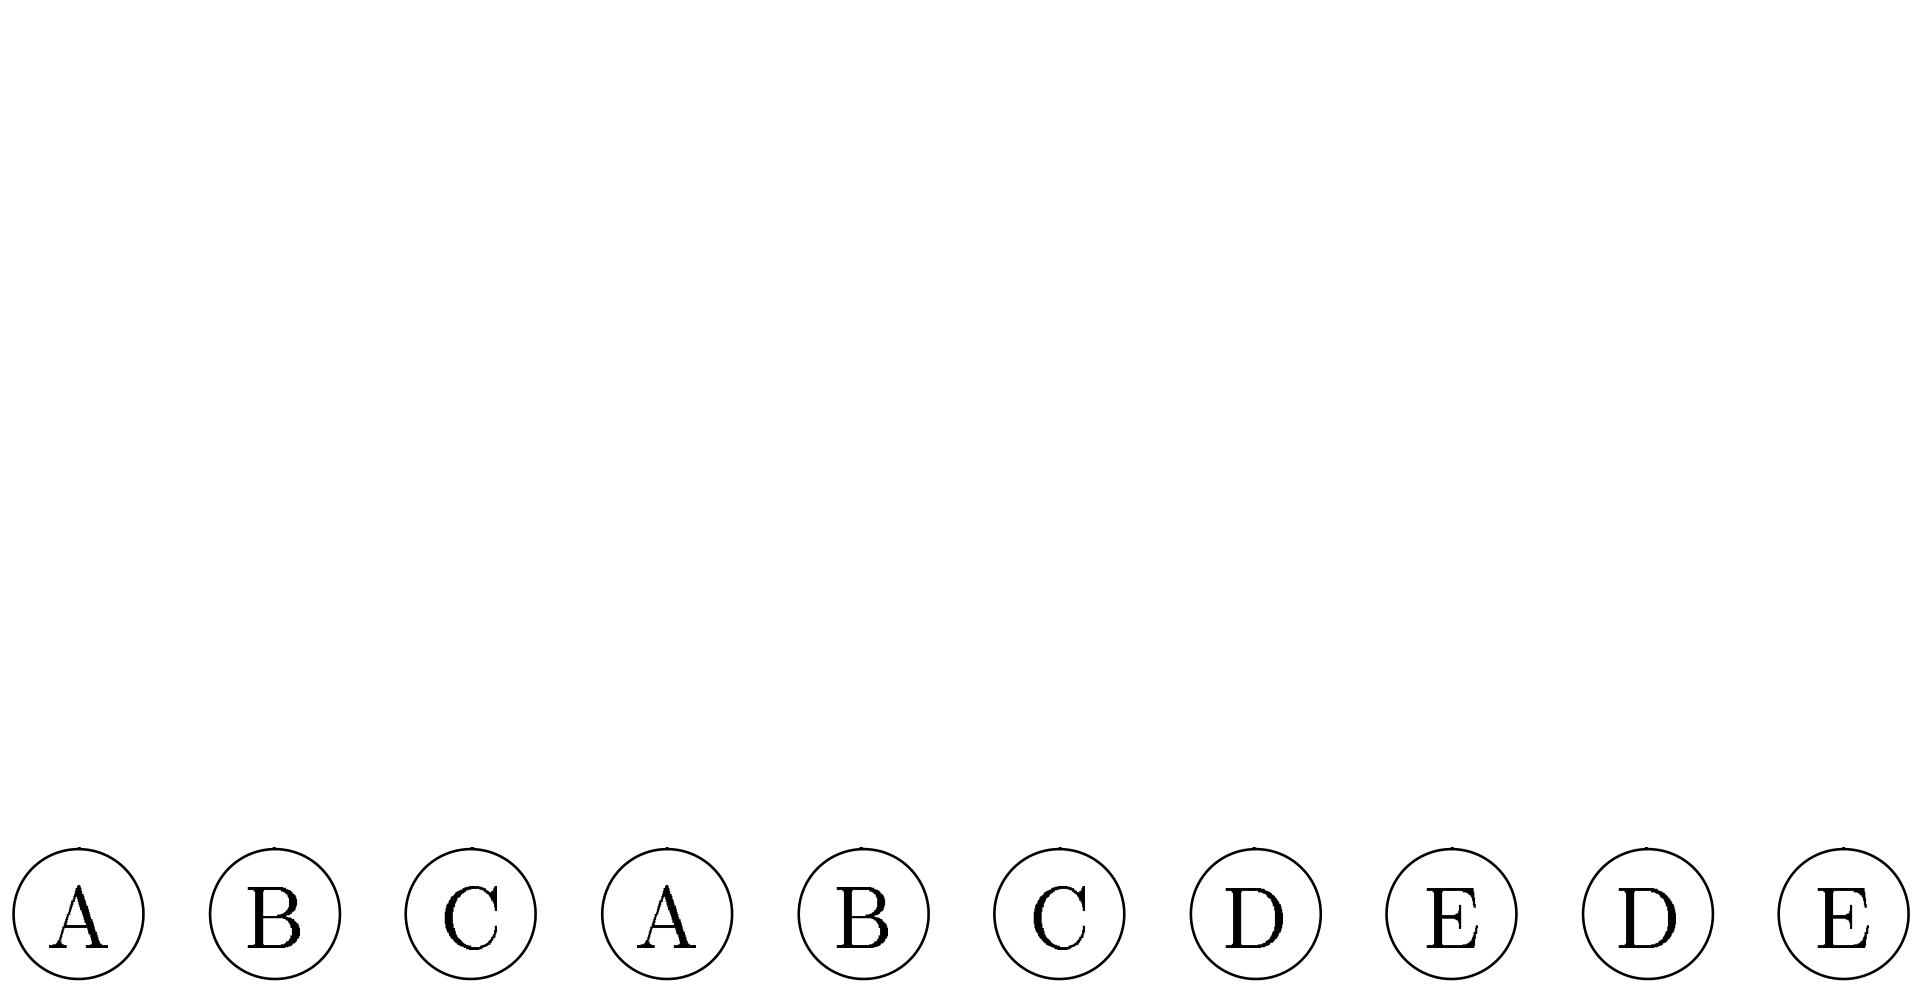
\includegraphics[scale=0.17]{creacionInc.jpg}
\end{figure}}
\pause
  \only<2>{\begin{figure}[h!]
    \centering
    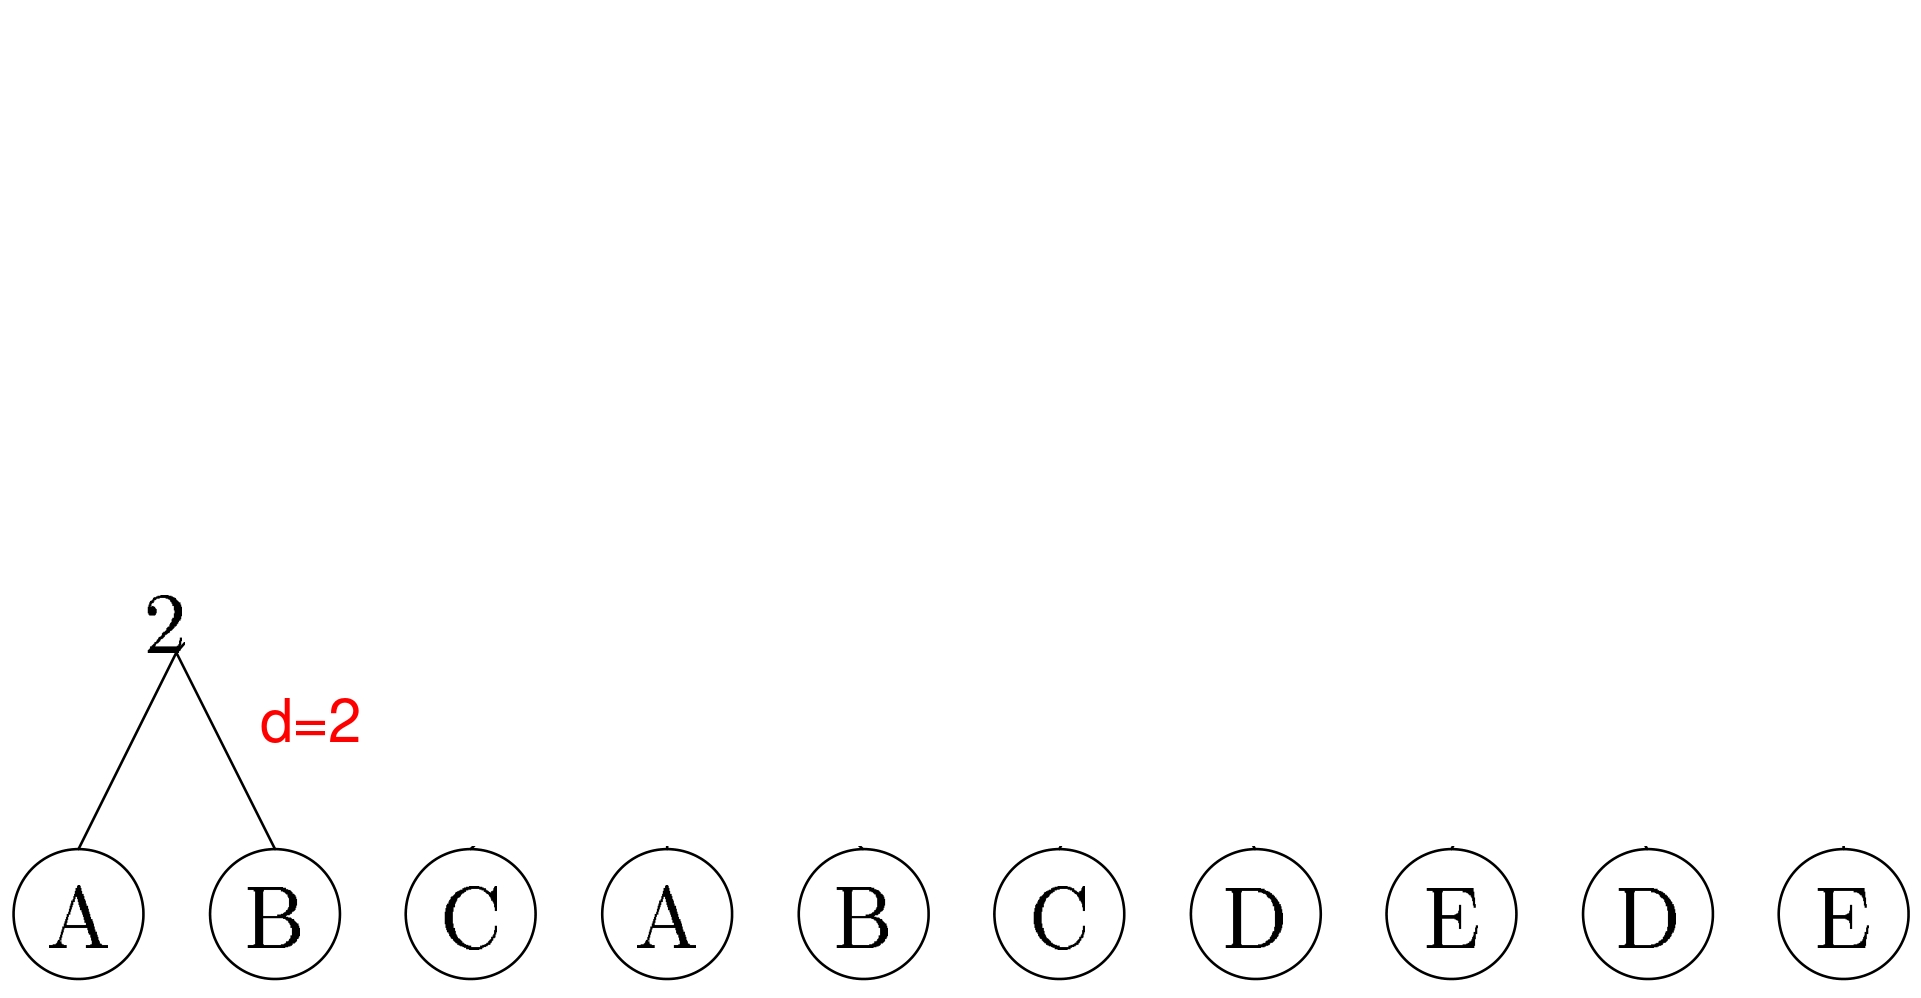
\includegraphics[scale=0.17]{creacion1.jpg}
\end{figure}}
\pause
  \only<3>{\begin{figure}[h!]
    \centering
    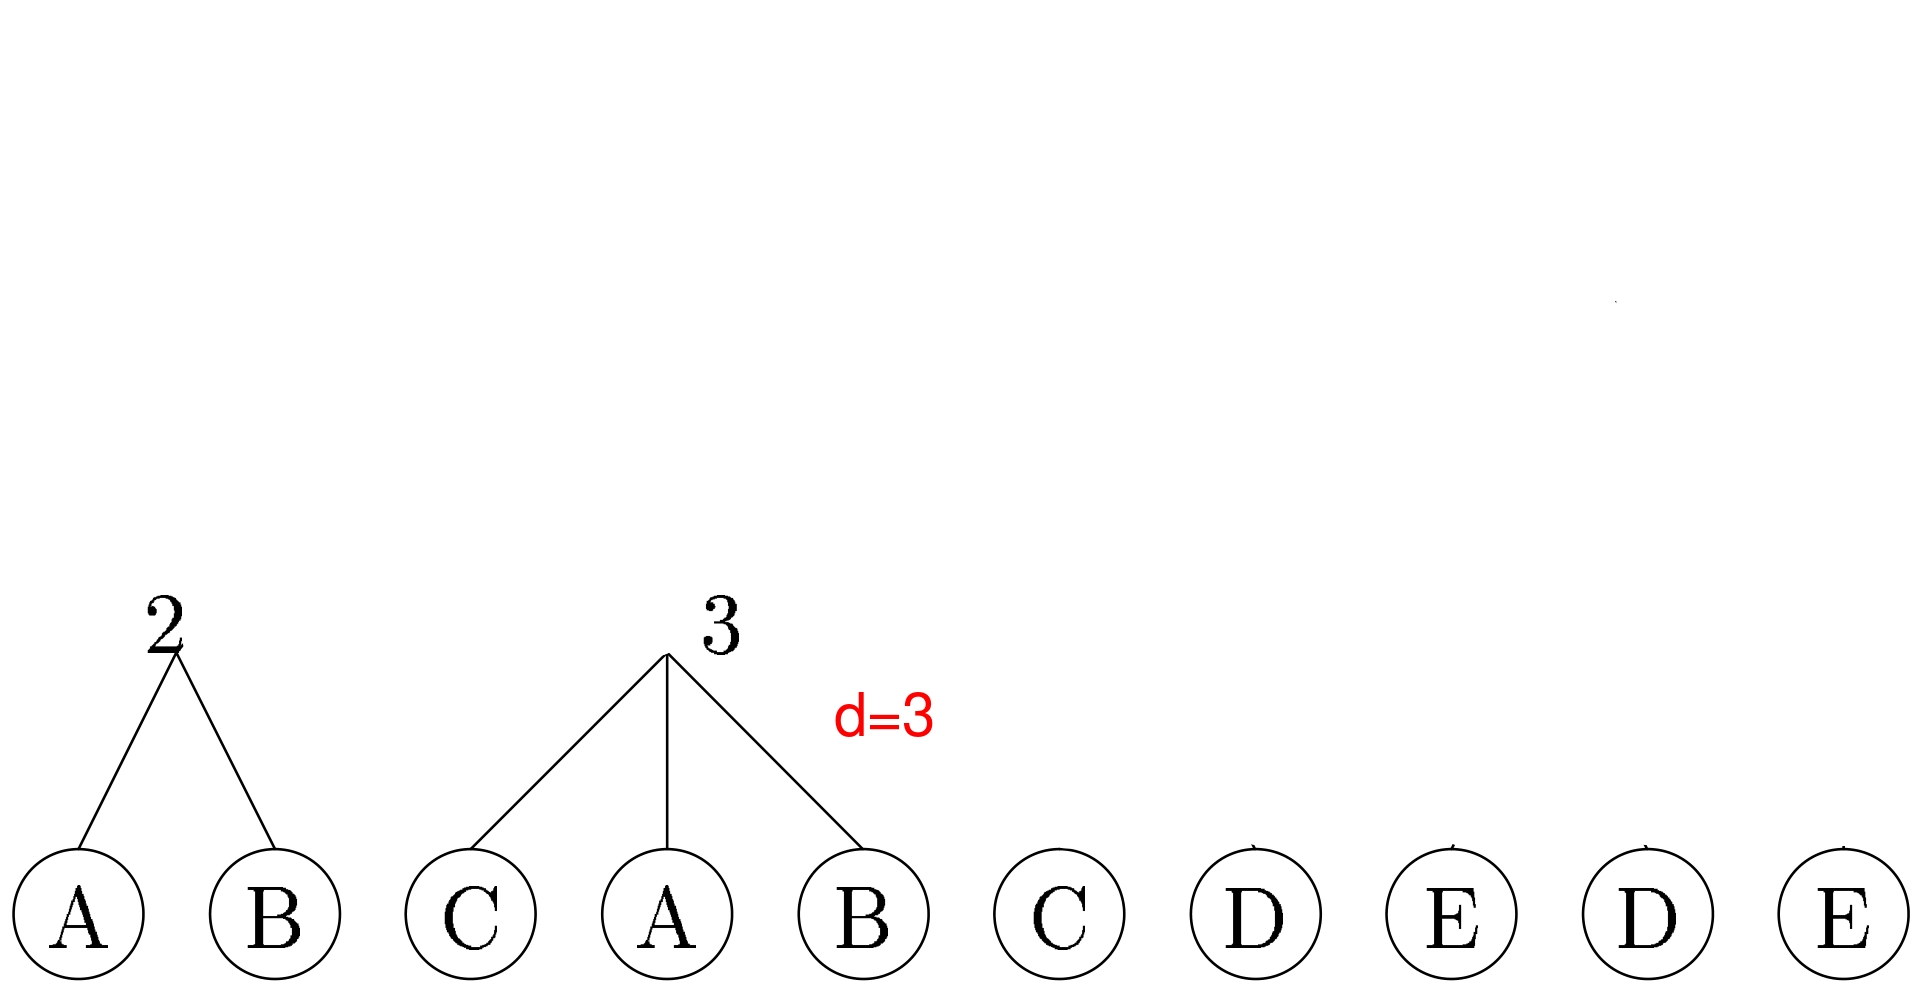
\includegraphics[scale=0.17]{creacion2.jpg}
\end{figure}}
  \pause
  \only<4>{\begin{figure}[h!]
    \centering
    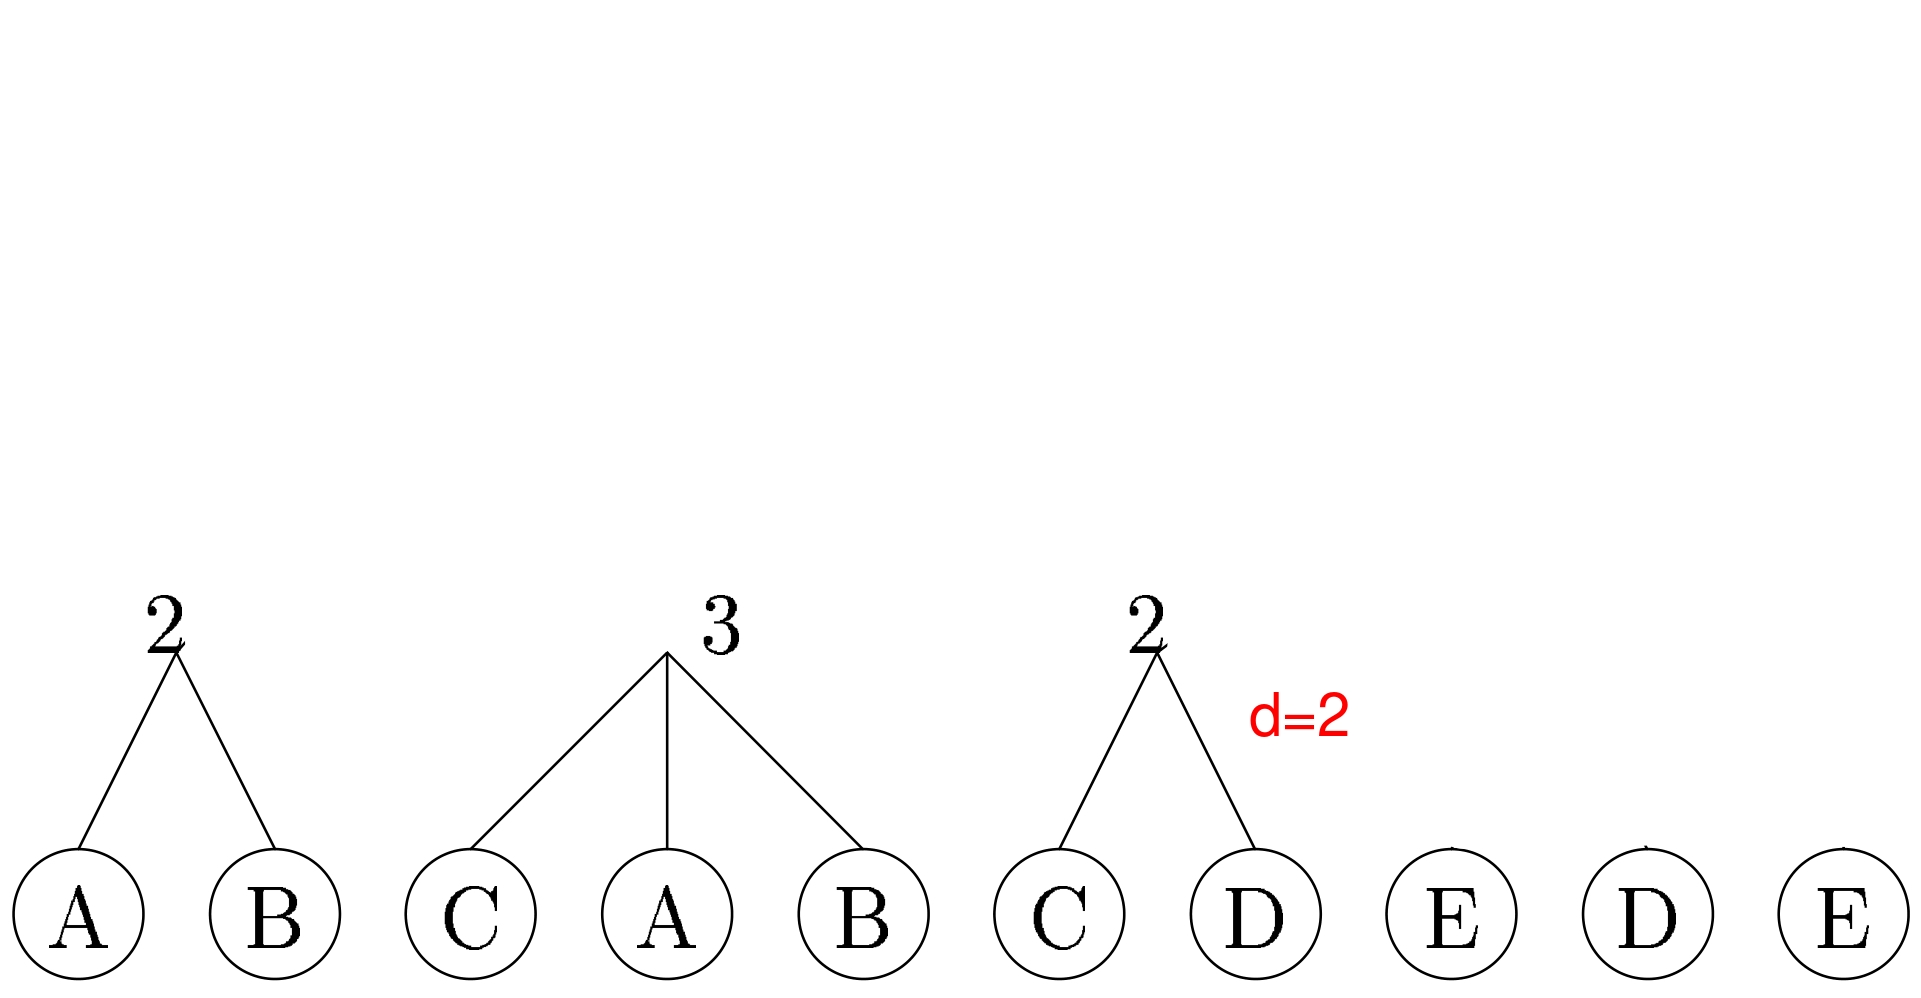
\includegraphics[scale=0.17]{creacion3.jpg}
\end{figure}}
  \pause
  \only<5>{\begin{figure}[h!]
    \centering
    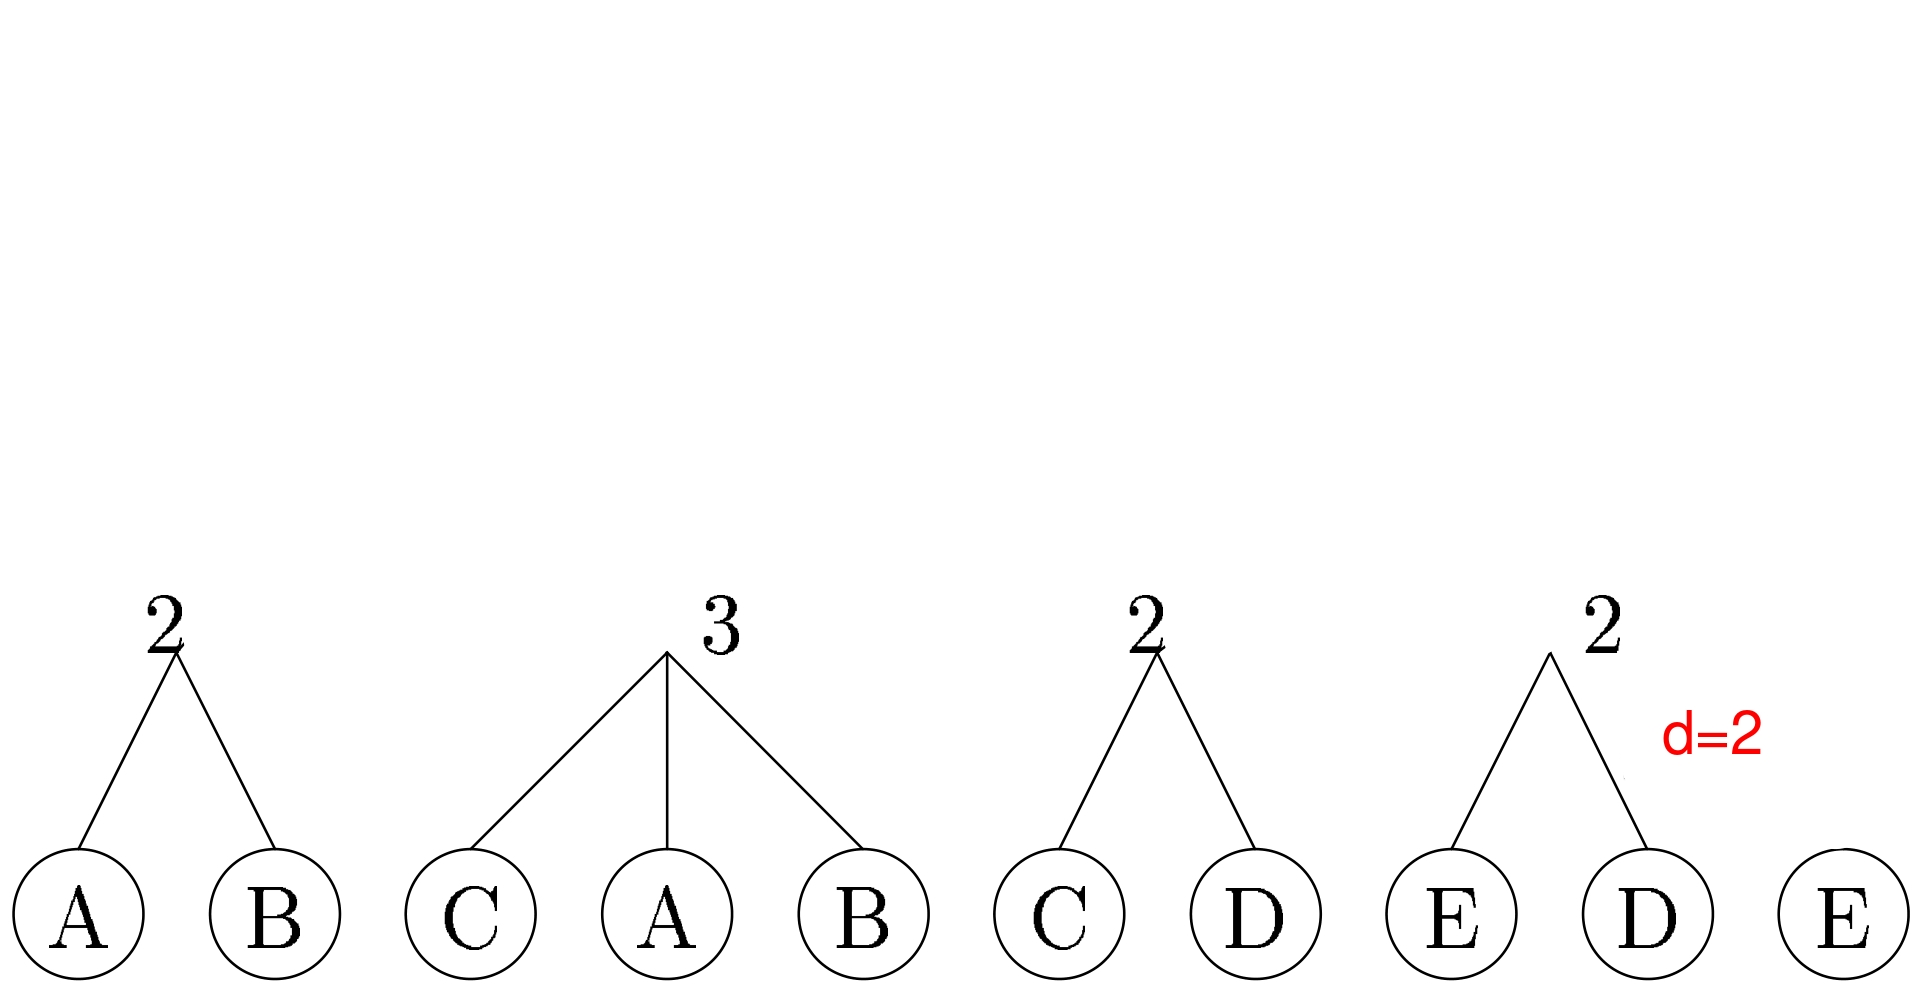
\includegraphics[scale=0.17]{creacion4.jpg}
\end{figure}}
  \pause
  \only<6>{\begin{figure}[h!]
    \centering
    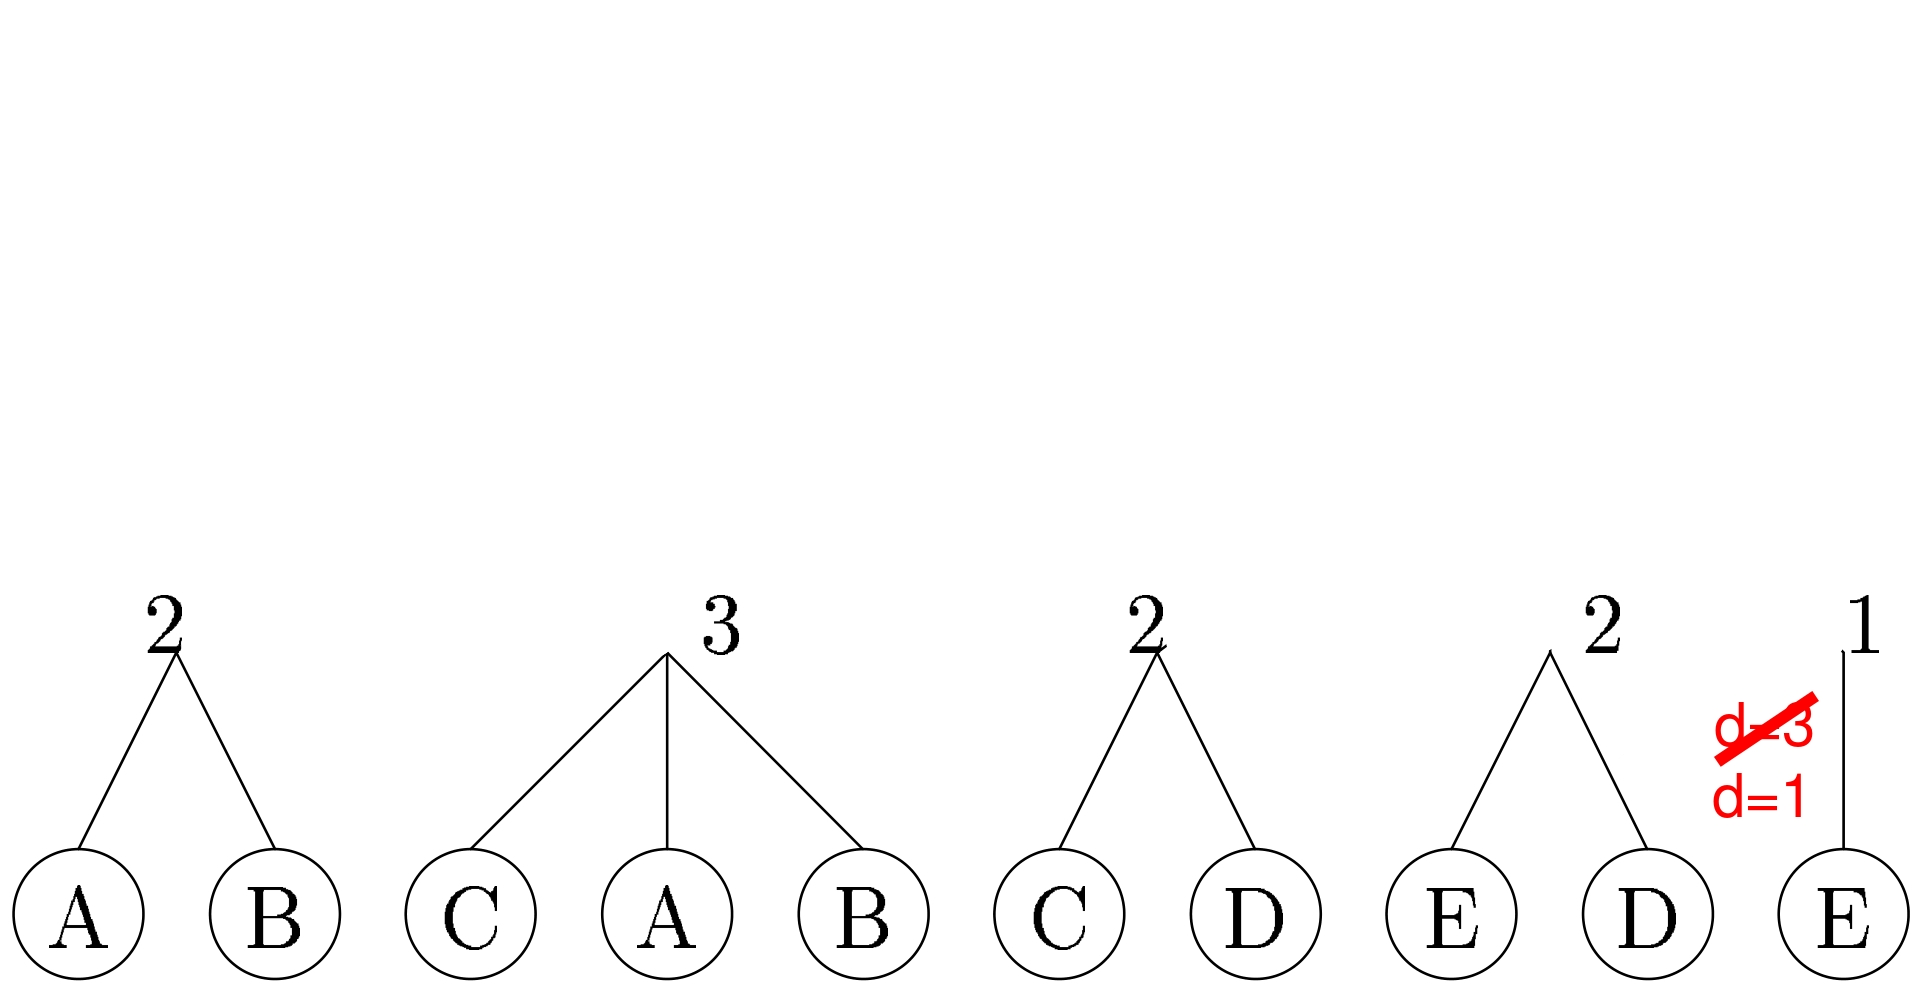
\includegraphics[scale=0.17]{creacion5.jpg}
\end{figure}}
  \pause
  \only<7>{\begin{figure}[h!]
    \centering
    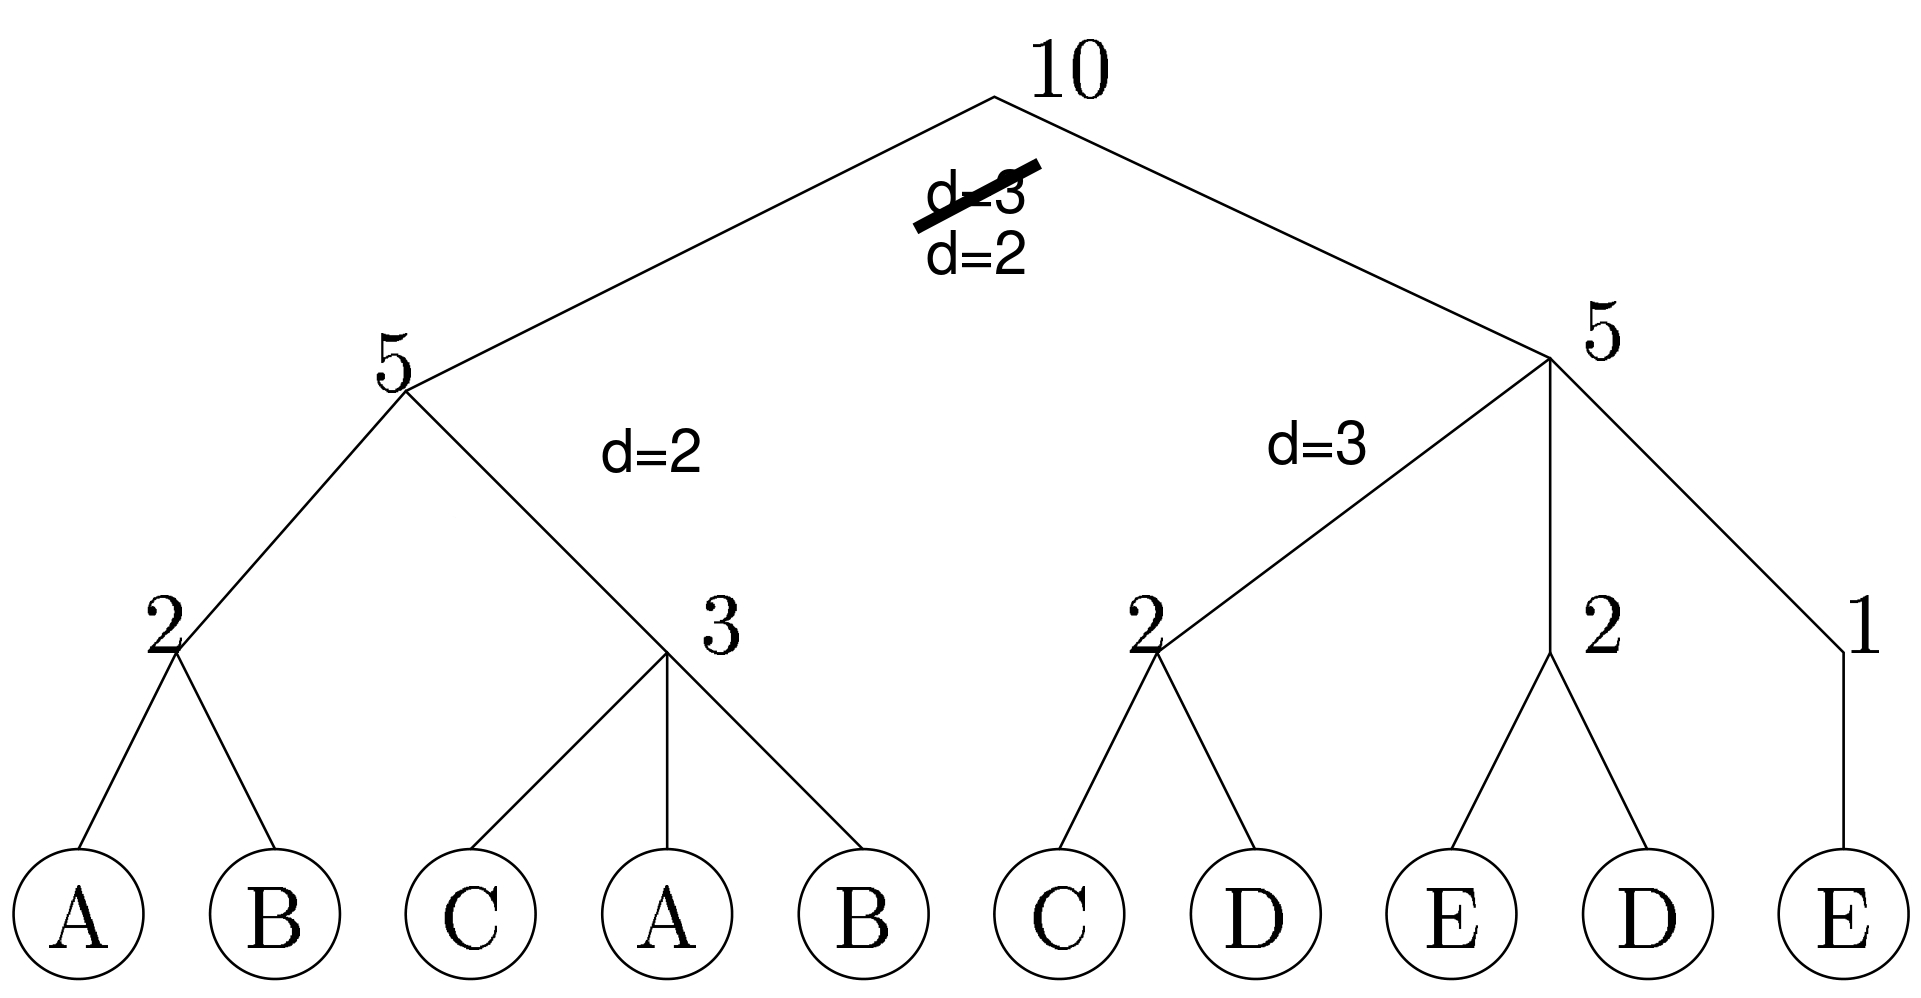
\includegraphics[scale=0.17]{creacion6.jpg}
\end{figure}}

\end{frame}

%%%%%%%%%%%%%%%%%%%%%%%%%%%%%%%%%%%%%%%%%%%%%%%%%%%%%%%%%%%%%%%%%%%%%%%%%%%%%%%%%%%%%%%%%%%%%%%%%%%%

\begin{frame}
\frametitle{Algoritmo Insertar}
  \texttt{Insertar}(i,b, T): Inserto el nodo hoja en la i-esima posicion y los nodos que le siguen son agrupados
  como se hace con  \texttt{Crear} hasta que se sincroniza con el arbol.

  Son dos loops anidados.

  Tiempo: O(logn)
\end{frame}



%%%%%%%%%%%%%%%%%%%%%%%%%%%%%%%%%%%%%%%%%%%%%%%%%%%%%%%%%%%%%%%%%%%%%%%%%%%%%%%%%%%%%%%%%%%%%%%%%%%%

\begin{frame}
\frametitle{Algoritmo Insertar}
 \begin{enumerate}\itemsep-1em
  \item Inserto hoja en la i-esima posicion.
  \item Loop en l: voy de l=h-1 hasta l=0.
    Donde h es la altura del arbol y $u_l$ el nodo del camino raiz a hoja en el nivel l.
    \vspace{-0.4cm}
    \begin{enumerate}[a]\itemsep-1em
    \item Si $u_l$ es el ultimo: Si $deg(u_l)=2$ listo, si $deg(u_l)=3$, se tira moneda $d$, si sale 3 listo. Recalculo los sizes.
      Si $deg(u_l)=3$ pero $d=2$ se continua al siguiente caso.
    \item Inicializo w=1 y termina con w=0 (loop en nivel l).
          \vspace{-0.4cm}
      \begin{enumerate}[i]\itemsep-1em
        \item Tiro moneda d para el grado del nodo vecino derecho a $u_l$.
        \item Transfiero los ultimos w hijos de $u_l$ al vecino (si no existe lo creo).
        \item Actualizo como w=max(0, t+w-d), donde t es el grado del nodo vecino originalmente y d lo que salio la moneda.
         \item Se recomputan los tama\~nos de los nodos insertados.
      \end{enumerate}
  \end{enumerate}
  \item  Recomputa el camino desde la raiz hasta la hoja insertada.
  Si la raiz tiene nuevo vecino, creo nueva raiz.
\end{enumerate}

\end{frame}

%%%%%%%%%%%%%%%%%%%%%%%%%%%%%%%%%%%%%%%%%%%%%%%%%%%%%%%%%%%%%%%%%%%%%%%%%%%%%%%%%%%%%%%%%%%%%%%%%%%%

\section{}
\begin{frame}
\frametitle{Ejemplo Insertar}
Ejemplo: \texttt{Insertar}(1, B, \texttt{Crear}(ACDE)).

  \only<1>{\centering Las dos unicas posibilidades de \texttt{Crear}(ACDE).
    \begin{figure}[h!]
    \centering
    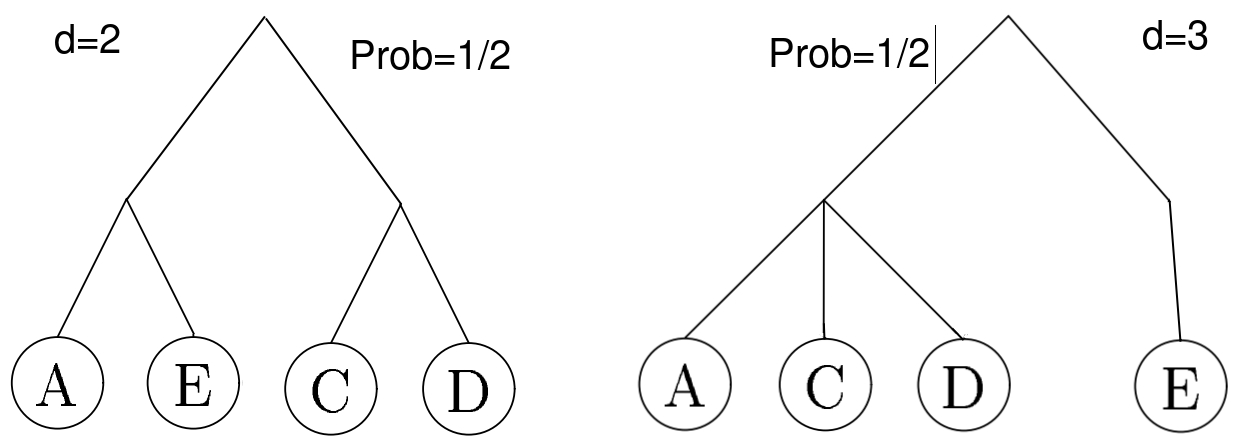
\includegraphics[scale=0.27]{insertCreate.jpg}
\end{figure}}
\pause
  \only<2>{\centering primer caso
    \begin{figure}[h!]
    \centering
    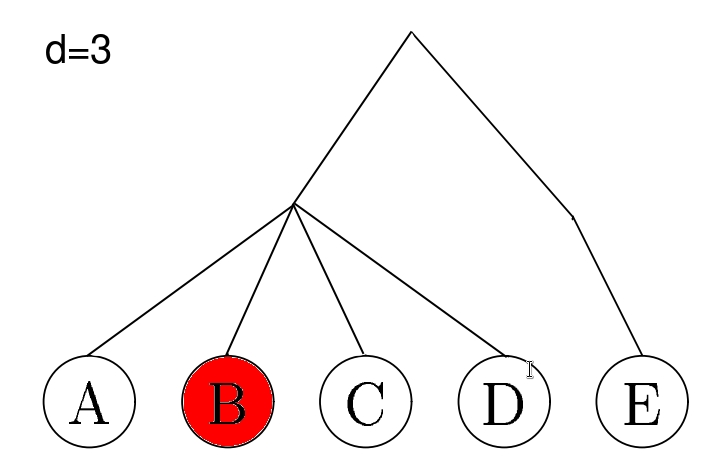
\includegraphics[scale=0.32]{insertCreateB0.jpg}
\end{figure}\centering
w=1 voy a pasarle un hijo, e independiente del d termina en 2ai/ii}
\pause
  \only<3>{\begin{figure}[h!]
    \centering
    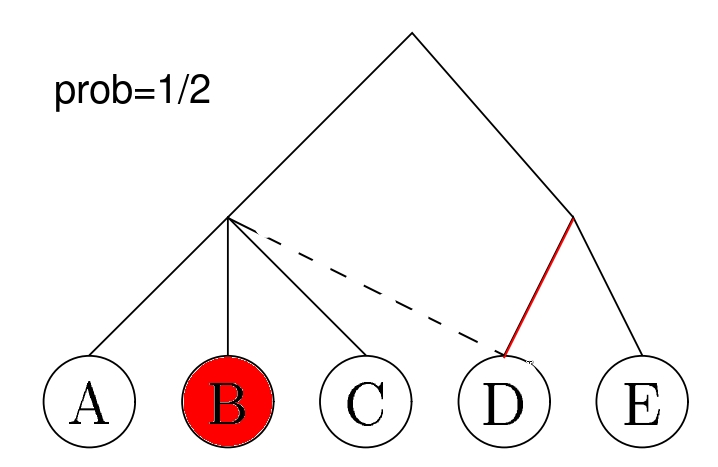
\includegraphics[scale=0.37]{insertCreateB1.jpg}
\end{figure}}
  \pause
  \only<4>{\centering segundo caso
    \begin{figure}[h!]
    \centering
    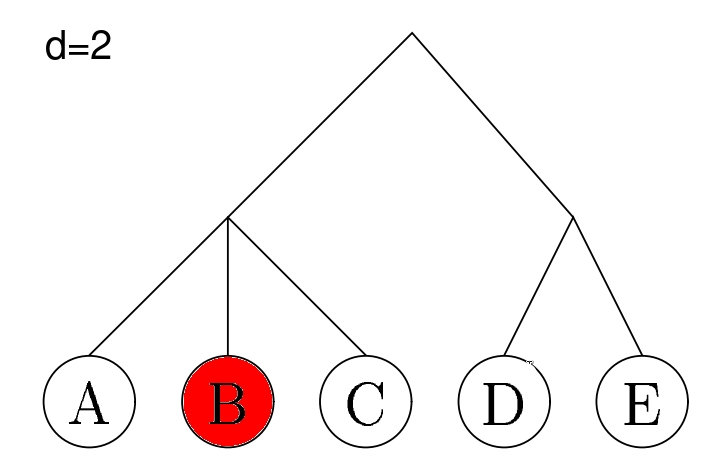
\includegraphics[scale=0.37]{insertCreateA0.jpg}
\end{figure}
\centering w=1, pasa un  hijo pero importa el d}
  \pause
  \only<5>{\centering caso d=2
    \begin{figure}[h!]
    \centering
    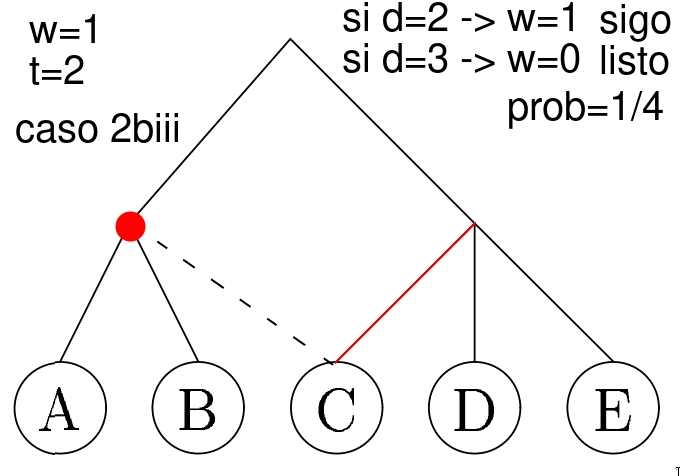
\includegraphics[scale=0.37]{insertCreateA1.jpg}
\end{figure}}
  \pause
  \only<6>{\centering caso d=2 nuevamente
   \begin{figure}[h!]
    \centering
    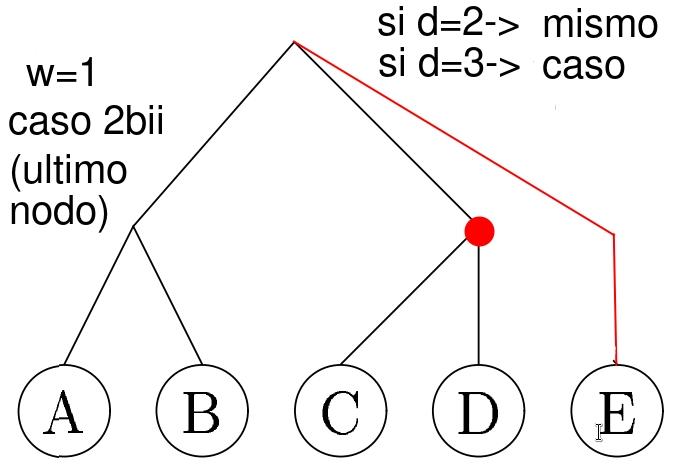
\includegraphics[scale=0.37]{insertCreateA2.jpg}
\end{figure}}
  \pause
  \only<7>{\centering Paso al nivel l-1
    \begin{figure}[h!]
    \centering
    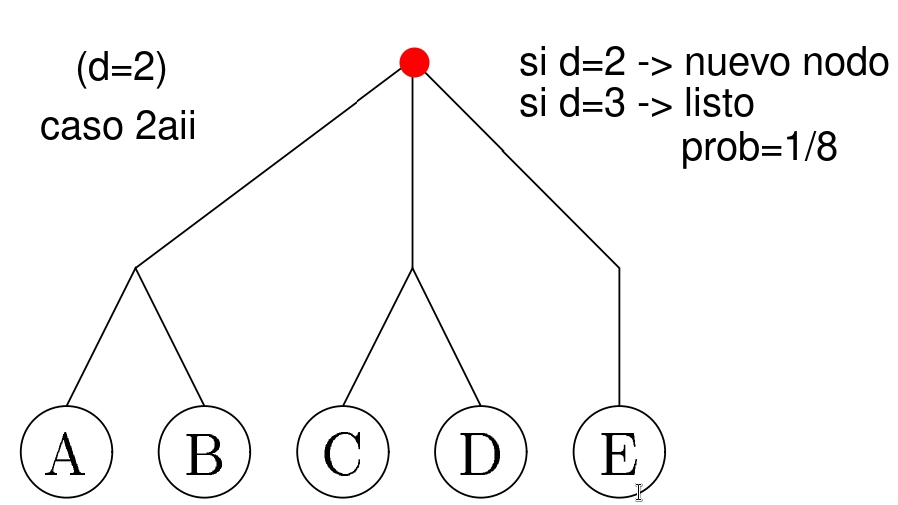
\includegraphics[scale=0.37]{insertCreateA3.jpg}
\end{figure}}
  \only<8>{\begin{figure}[h!]
    \centering
    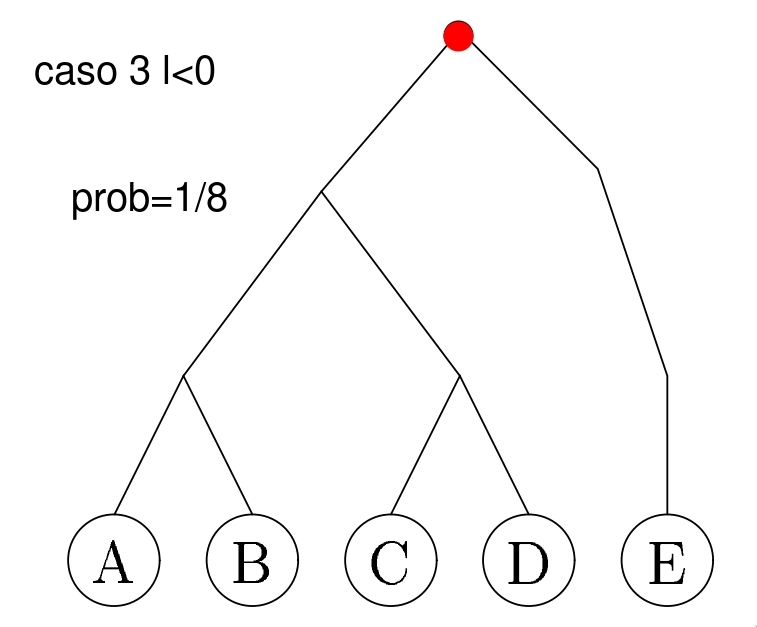
\includegraphics[scale=0.37]{insertCreateA4.jpg}
\end{figure}}



\end{frame}


%%%%%%%%%%%%%%%%%%%%%%%%%%%%%%%%%%%%%%%%%%%%%%%%%%%%%%%%%%%%%%%%%%%%%%%%%%%%%%%%%%%%%%%%%%%%%%%%%%%%

\section{}
\begin{frame}
\frametitle{Borrado}
\texttt{Borrar}(i, T): Borro el nodo hoja de la i-esima posicion y los nodos que le siguen son agrupados
  como se hace con  \texttt{Crear} hasta que se sincroniza con el arbol.

  Son dos loops anidados. Muy similar al Insertar, misma nomenclatura.

  Tiempo: O(logn)

\end{frame}
%%%%%%%%%%%%%%%%%%%%%%%%%%%%%%%%%%%%%%%%%%%%%%%%%%%%%%%%%%%%%%%%%%%%%%%%%%%%%%%%%%%%%%%%%%%%%%%%%%%%

\begin{frame}
\frametitle{Algoritmo Borrar}

 \begin{enumerate}\itemsep-1em
  \item Loop en l: voy de l=h-1 hasta l=0.
    Donde h es la altura del arbol y $u_l$ el nodo del camino raiz al nodo en el nivel l a remover.
    \vspace{-0.4cm}
    \begin{enumerate}[a]\itemsep-1em
    \item Borro $u_{l+1}$ de los hijos de $u_l$.
    \item Si $u_l$ es el ultimo: Si $u_{l=1}$ es el unico hijo de $u_l$ paso a la siguiente iteracion, caso contrario
      voy al paso 3.
    \item Inicializo w=1 y termina con w=0 (loop en nivel l).
          \vspace{-0.4cm}
      \begin{enumerate}[i]\itemsep-1em
        \item t=$deg(u_l)$, si $w\geq t$ cambio los hijos del vecino derecho a $u_l$ y pongo w=0 y recomputo  tama\~nos.
        \item Tiro moneda d.
        \item Transfiero los  primeros w hijos del vecino derecho a $u_l$.
        \item Actualizo como w=max(0, d-t+w).
        \item Se recomputan los tama\~nos de los nodos modificados.
      \end{enumerate}
  \end{enumerate}
  \item  Recomputa el camino desde la raiz hasta la hoja insertada.
  Si la raiz tenia 2 hijos y borre 1, hago a su unico hijo la raiz y borro la raiz original.
\end{enumerate}
\end{frame}
%%%%%%%%%%%%%%%%%%%%%%%%%%%%%%%%%%%%%%%%%%%%%%%%%%%%%%%%%%%%%%%%%%%%%%%%%%%%%%%%%%%%%%%%%%%%%%%%%%%%
\section{}
\begin{frame}
\frametitle{Calculo de complejidad}

Calculo \texttt{Insertar} y \texttt{Borrar} similares.
Calculamos el primero.
Rec: Tiempo esperado O(logn).
\vspace{-0.2cm}

Parte critica del algoritmo el loop anidado. El loop principal como mucho puede
correrse h=O(logn) veces.
\vspace{-0.2cm}

Dem que w Solo toma valores {0,1,2}. Rec: w inicializa con 1 y si $d\neq w$ w=max{0, t+w-d}. $t\in{1,2,3}$ y $d\in{2,3}$
Trivialmente se comprueba.
\vspace{-0.2cm}

Lema: en cada iteracion de este loop, hay proba 1/4 de setear w=0 (y asi terminar el loop) dentro de 2 iteraciones.
\vspace{-0.2cm}

Dem: en cada iteracion $w\in{2,3}$. Si $u_l$ es el ultimo nodo w=0.
Si no, podemos tener w=2 y con proba 1/2 sacar d=2 y terminar.
Si tenemos w=1 tenemos dos casos.
\vspace{-0.3cm}
\begin{itemize}\itemsep-1em
  \item t=2: con proba 1/2 tenemos d=3 y entonces w=t+w-d=0, termino.
  \item t=3: con proba 1/2 tenemos d=2 y actualizamos  w=t+w-d=2, que en la siguiente
    iteracion seteamos w=0 con probabilidad 1/2.
\end{itemize}
\end{frame}

%%%%%%%%%%%%%%%%%%%%%%%%%%%%%%%%%%%%%%%%%%%%%%%%%%%%%%%%%%%%%%%%%%%%%%%%%%%%%%%%%%%%%%%%%%%%%%%%%%%%

\section{}
\begin{frame}
\frametitle{Misma distribucion de probabilidad.}

Queremos probar que para toda secuencia $L=L[1]L[2]...L[n]$, y sea $i\leq n$ y b una clave,
loas siguientes igualidades se cumplem para las distribuciones de probabilidad.

\begin{centering}
  \texttt{Insertar}(i,b, \texttt{Crear}(L))=\texttt{Crear}(L[1],...,L[i],b,L[i+1],...,L[n])
\end{centering}

\begin{centering}
  \texttt{Borrar}(i \texttt{Crear}(L))=\texttt{Crear}(L[1],...,L[i-1],L[i+1],...,L[n])
\end{centering}

Dem primer caso, segundo caso analogo.

Por un lado en cada iteracion $l$ solo se cambia la topologia de ese nivel y que
hasta el hijo en cuestion no se modifica su agrupado con el algoritmo de \texttt{Insertar}.
Los siguientes nodos son modificados de la misma forma que \texttt{Crear} pero con
monedas diferentes e independientes.
Esto genera que tengan mismas distribuciones de probabilidad.

\end{frame}

%%%%%%%%%%%%%%%%%%%%%%%%%%%%%%%%%%%%%%%%%%%%%%%%%%%%%%%%%%%%%%%%%%%%%%%%%%%%%%%%%%%%%%%%%%%%%%%%%%%%

\section{}
\begin{frame}
\frametitle{Ejemplo probabilidades}

Ejemplo con \texttt{Crear}(ABCDE) y \texttt{Insertar}(1, B, \texttt{Crear}(ACDE)).

Para el caso de insertar ya lo hicimos \texttt{Insertar} y nos dio lo siguiente:

\begin{figure}[h!]
    \centering
    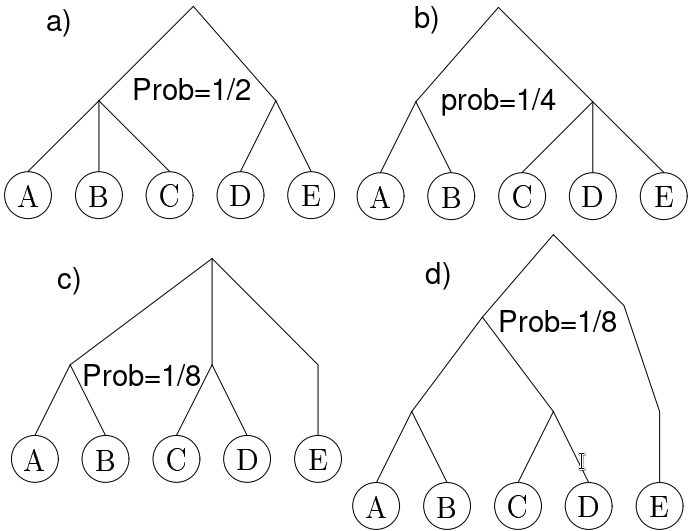
\includegraphics[scale=0.3]{insertCreateRes.jpg}
\end{figure}

\end{frame}

%%%%%%%%%%%%%%%%%%%%%%%%%%%%%%%%%%%%%%%%%%%%%%%%%%%%%%%%%%%%%%%%%%%%%%%%%%%%%%%%%%%%%%%%%%%%%%%%%%%%

\section{}
\begin{frame}
\frametitle{Ejemplo probabilidades}

Basta con probar que \texttt{Crear}(ABCDE) tiene las mismas probabilidades.

\begin{itemize}
  \item Primer caso, d=3 prob 1/2, termina (caso a). \pause
  \item Segundo caso d=2, prob 1/2, sigue en el siguiente nodo:
    \begin{itemize}\pause
      \item d=3, con prob 1/2*1/2=1/4, termina (caso b).\pause
      \item d=2, prob 1/2*1/2=1/4, termina en ese nivel pero sigue en el proximo:
        \begin{itemize}\pause
          \item d=3, prob 1/4*1/2=1/8, termina (caso c).\pause
          \item d=2, prob 1/4*1/2=1/8, crea un nodo al lado de la raiz. Se crea
            un nuevo nivel con nueva raiz.
        \end{itemize}
    \end{itemize}
\end{itemize}

\pause

Comprobado!

\end{frame}

%%%%%%%%%%%%%%%%%%%%%%%%%%%%%%%%%%%%%%%%%%%%%%%%%%%%%%%%%%%%%%%%%%%%%%%%%%%%%%%%%%%%%%%%%%%%%%%%%%%%

\section{}
\begin{frame}
\frametitle{}

\huge
\centering
FIN!
\end{frame}

%%%%%%%%%%%%%%%%%%%%%%%%%%%%%%%%%%%%%%%%%%%%%%%%%%%%%%%%%%%%%%%%%%%%%%%%%%%%%%%%%%%%%%%%%%%%%%%%%%%%

\section{}
\begin{frame}
\frametitle{Algoritmo insertar completo}
\small
\begin{enumerate}\itemsep0em
  \item Localizo la i-esima hoja e inserto el valor. Sea $u_0,...,u_h$ el camino
    de la raiz a la nueva hoja.
  \item Repetimos los siguientes pasos de l=h-1,h-2,...,0. Donde en cada iteracion
    es de la raiz al nuevo nodo.
    \vspace{-0.05cm}
    \begin{enumerate}[a]\itemsep0em
      \item Si $u_l$ es el ultimo nodo del nivel l:
        \vspace{-0.05cm}
        \begin{enumerate}[i]\itemsep0em
          \item Si $u_l$ tiene grado 2 entonces ir al paso 3.
          \item Si $u_l$ tiene grado 3, elijo de forma uniforme $d\in{2,3}$ y si
            $d=4$ ir al paso 3, si no continuar.
        \end{enumerate}
      \item Inicializamos la variable w=1 y repetimos los pasos hasta w=0:
        \vspace{-0.05cm}
        \begin{enumerate}[i]\itemsep0em
          \item Sea $u_l'=u_l$ y elegimos de forma uniforme $d\in{2,3}$. d es el grado
            del nodo que sigue a $u_l'$.
          \item Si d=w o si $u_l'$ es el ultimo nodo al nivel l, insertamos el nuevo nodo $u_l$
            a la derecha de $u_l'$, seteamos w=0 y vamos al paso 2(b)v.
          \item En caso contrario, hacemos $u_l$ el nodo que continua a $u_l'$ en el nivel l y
            sea t=deg($u_l$) (el que tenia de antes).
          \item Cambiamos de padre los ultimos $w$ hijos de $u_l'$ a $u_l$ y hacemos $w=max(0, t+w-d)$.
          \item Recomputamos el tama\~no de los nodos a lo largo del camino de $u_l'$ a $u_l$ no incluido.
        \end{enumerate}
    \end{enumerate}
  \item Si $l\geq$0, recomputamos la informacion de tama/~no de los nodos del camino.
    En caso contrario aumentamos la altura del arbol en uno creando un nuevo nodo raiz
    y hacemos de hijos $u_0'$ y el nuevo nodo $u_0$
\end{enumerate}

\end{frame}
%%%%%%%%%%%%%%%%%%%%%%%%%%%%%%%%%%%%%%%%%%%%%%%%%%%%%%%%%%%%%%%%%%%%%%%%%%%%%%%%%%%%%%%%%%%%%%%%%%%%

\section{}
\begin{frame}
\frametitle{Algoritmo borrar completo}
\small
\begin{enumerate}\itemsep0em
  \item Localizo la i-esima hoja e inserto el valor. Sea $u_0,...,u_h$ el camino
    de la raiz a la nueva hoja.
  \item Repetimos los siguientes pasos de l=h-1,h-2,...,0. Donde en cada iteracion
    es de la raiz al nuevo nodo.
    \vspace{-0.05cm}
    \begin{enumerate}[a]\itemsep0em
      \item Si $u_l$ es el ultimo nodo del nivel l:
        \vspace{-0.05cm}
      \item Borramos $u_{l+1}$ de los hijos de $u_l$.
      \item Si $u_l$ es el ultimo nodo del nivel: Si $u_{l+1}$ era el unico hijo de $u_l$
      , continuamos con la siguiente iteracion del loop 2, si no al paso 3.
      \item Inicializamos la variable w=1 y repetimos los pasos hasta w=0:
        \vspace{-0.05cm}
        \begin{enumerate}[i]\itemsep0em
          \item Sea $u_l'=u_l$ y movemos para adelante $u_l$.
          \item Hacemos t=deg($u_l$). Si $w\geq t$, cambiamos los paodres de los hijos de $u_l$
            a $u_l'$, seteamos w=0 y vamos al paso 2(c)v.
          \item Elegimos de forma uniforme $d\in{2,3}$.
          \item Cambiamos de padre los primeros $w$ hijos de $u_l'$ a $u_l$ y hacemos $w=d-t+w)$.
          \item Recomputamos el tama\~no de los nodos a lo largo del camino de $u_l'$ a $u_l$ no incluido.
        \end{enumerate}
    \end{enumerate}
  \item Si $l\geq$0, recomputamos la informacion de tama/~no de los nodos del camino.
    En caso contrario borramos el nodo $u_0$ y hacemos $u_1$ la nueva raiz del arbol.
\end{enumerate}

\end{frame}
%%%%%%%%%%%%%%%%%%%%%%%%%%%%%%%%%%%%%%%%%%%%%%%%%%%%%%%%%%%%%%%%%%%%%%%%%%%%%%%%%%%%%%%%%%%%%%%%%%%%



\end{document}

